\chapter{Métricas}

\section{Processo de Medição}

	Medição é o mapeamento de relações empíricas em relações formais. Isto é, quantificação em símbolos com objetivo de caracterizar uma entidade por meio de seus atributos. \cite{Fenton98}.
	
	Segundo \citeonline{ISO:15939}, medição, que é uma ferramenta primordial para gerenciar as atividades do desenvolvimento de software e para avaliar a qualidade dos produtos e a capacidade de processos organizacionais,  é um conjunto de operações que visam por meio de um objeto determinar um valor a uma medida ou métrica.\footnote{A definição formal da \citeonline{ISO:15939} não utiliza o termo métrica, sendo que este é definido pelo GQM em \citeonline{Basili96b}, que é uma outra abordagem para medição, contudo compreende-se que o termo medida tem valor semântico equivalente ao de métrica no contexto do presente trabalho}. 
	
	
	O processo de medição da \citeonline{ISO:15939}, como é mostrado na figura \ref{processo}, consiste  de quatro atividades que são sequenciadas em um ciclo iterativo, permitindo
	feedback e melhoria contínua do processo. Ele é uma adaptação do ciclo PDCA (Plan-Do-Check-Act), comumente utilizado como base para a melhoria da qualidade \cite{Barcellos2010}.  O processo visa a construção de produtos de informação para cada necessidade seguindo um modelo de informação, que é mostrado na figura \ref{informacao}.
		
		\begin{figure}[h]
		\centering
		
			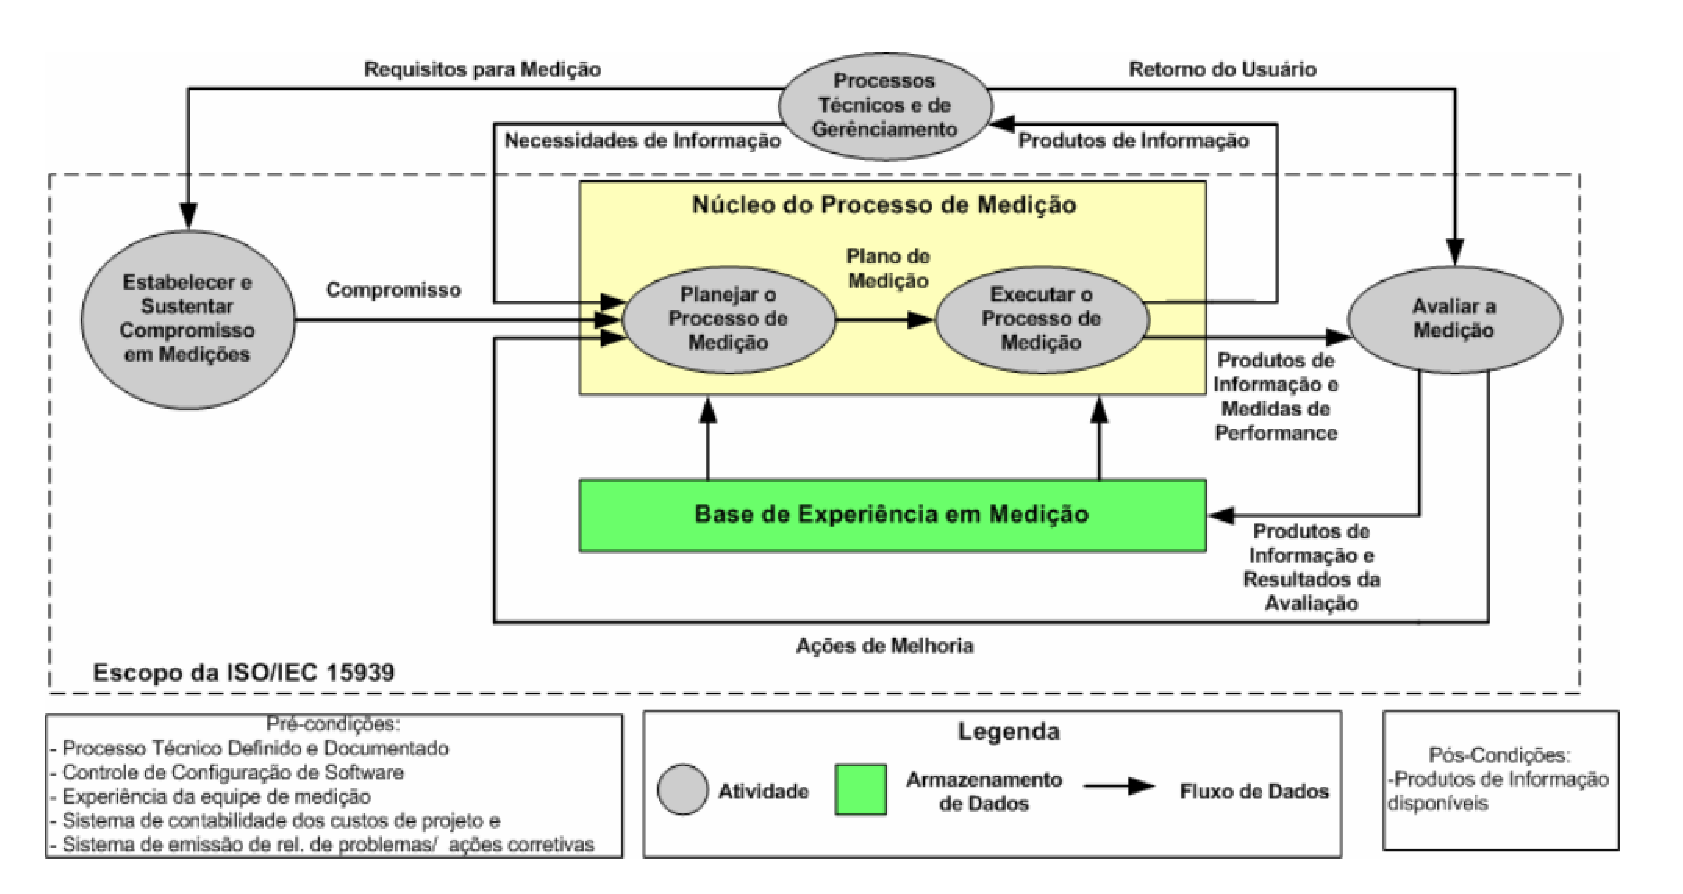
\includegraphics[keepaspectratio=true,scale=0.6]{figuras/processodemedicao15939.eps}
		\caption{Processo de Medição da ISO 15939 - Extraído de \cite{Gava2006}}
		\label{processo}
	\end{figure}
		

	\begin{figure}[h]
		\centering
		
			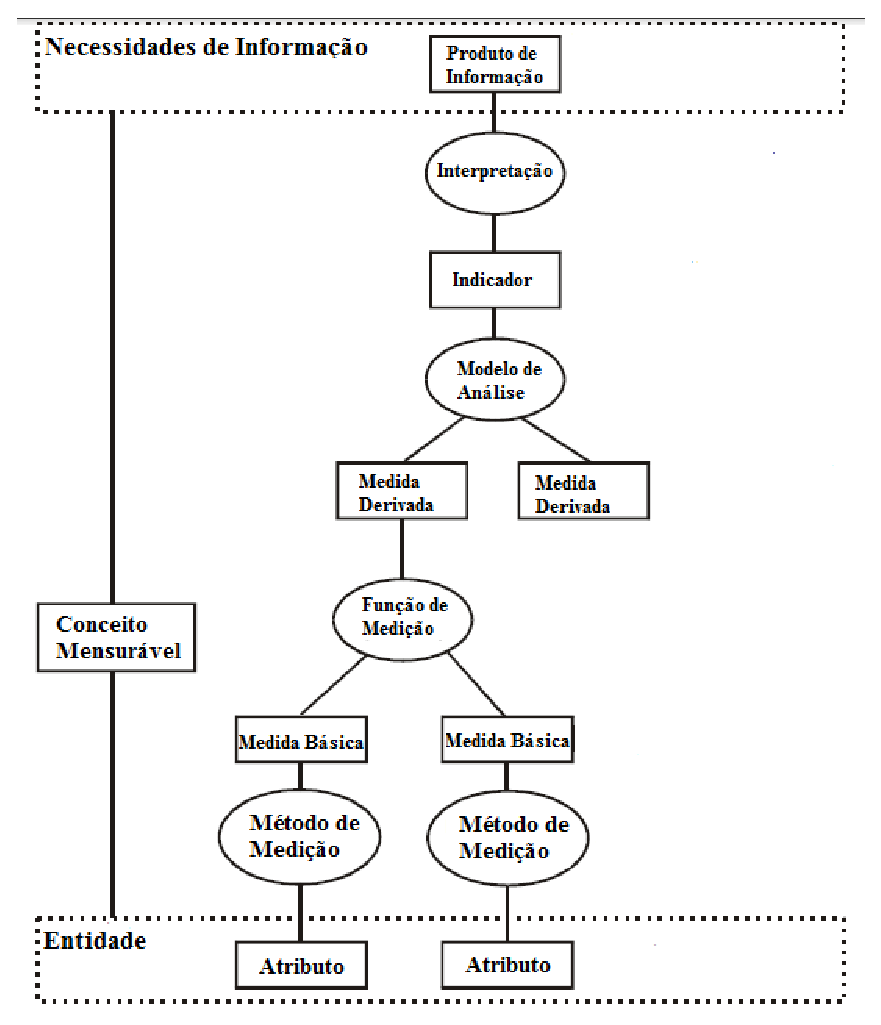
\includegraphics[keepaspectratio=true,scale=0.7]{figuras/modelodeinformacao15939.eps}
		\caption{Modelo de Informação da ISO 15939}
		\label{informacao}
	\end{figure}

		A terminologia do modelo de informação, que é mostrado na figura \ref{informacao} é descrito a seguir:
	\begin{description}
	%----------
	 \item [Necessidade de Informação.]  São situações as quais requer conhecimento de uma ou mais entidades para gerenciar objetivos, metas, riscos e problemas.
	
	%---------
	 \item [Entidade.]  Uma entidade é um objeto (como por exemplo, um processo, produto, projeto ou recurso) que é caracterizado por um atributo mensurável;
	%----------
	 \item [Atributo.]  Um atributo é uma propriedade ou característica de uma entidade que pode distiguí-la quantitativamente ou qualitativamente utilzando métodos manuais ou automáticos
	
	%----------
	 \item [Conceito Mensurável.]  Uma relação entre os atributos e as necessidades de informação. Como por exemplo, a qualidade de um produto. 
	 
	%----------
	 \item [Medida Básica ou Métrica Direta.] Uma medida básica é definida em termos do atributo e do método para sua quantificação, ou seja, é a variável a qual se atribui um valor. Cada medida básica é funcionalmente independente de outras medidas básicas e captura apenas um atributo. 
	%----------
	 \item [Método de Medição.] O método de medição é uma sequência de operações, descritas genericamente, usadas qualificar ou quantificar um atributo, ou seja, obter uma medida básica ou derivada com respeito a uma escala. Um método de medição pode ser classificado em:
	
		\begin{description}
		 \item [Subjetivo.] Envolve o julgamento humano. Resulta em medidas ou métricas subjetivas.
		 \item [Objetivo.] Baseado em regras númericas, tais como contagem. Pode ser realizado de forma manual ou automática. Resulta em medidas ou métricas objetivas.
		\end{description}
	%----------
	 \item [Escala.] Uma escala é um conjunto ordenado de valores, contínos ou discretos, ou uma série de categorias as quais um atributo é mapeado. O método de medição mapeia a magnitude, ou valor absoluto, de um atributo medido em um valor de escala. As escalas podem ser: 
	
		\begin{description}
			%----------
		 	\item [Nominal.] A medição é categórica. Por exemplo, a classificação dos tipos de defeitos. Nesta escala, só é possível realização de comparações.
			%----------
			\item [Ordinal.] A medição é baseada em ordenação. Por exemplo, a classificação das \textit{releases}. Nesta escala, é possível realizar ordenação de elementos.
			%----------
		 	\item [Intervalo.]A medição é baseada em distâncias iguais definidas para as menores unidade. Por exemplo, o aumentar de 1º C em um dia corresponde ao mesmo 1º C em outro dia qualquer. Nesta escala é possível realizar ordenação, soma e subtração.
			%----------
		 	\item [Racional.] A medição é baseada em distâncias iguais definidas para as menores unidades, e neste caso é possível a ausência por meio do zero absoluto. Como por exemplo, a quantidade de linhas de código em uma classe. Nesta escala, é possível realizar ordenação, soma, subtração, mutiplicação e divisão.
		\end{description}
	%----------
	 \item [Função de Medição.] Trata-se do algoritmo para combinar duas ou mais medidas básicas ou métricas diretas.
	%----------
	 \item [Medida Derivada ou Métrica Derivada.] Uma medida derivada ou métrica derivada é definida como uma função de medição de duas ou mais medidas básicas ou métricas diretas.
	
	 \item [Indicador.]  É uma medida que fornece uma estimativa ou avaliação de atributos especificados em relação a uma necessidade de informação. Um indicador inclui um ou mais valores de medidas básicas e/ou derivadas.

	\item [Interpretação.]  É a explicação dos indicadores, isto é, a interpretação que cada valor quantitativo do indicador mostra.
	
	\item [Produto de Informação] É o resultado esperado do processo de medição, que visa responder as necessidades de informação. O produto de informação pode vir a se materializar em forma de relatórios, gráficos ou planilhas.
	\end{description}


%---------------------------------------------------------------------------------------------------------------------%
	\section{Classificação das Métricas}	
	\label {Classificação das Métricas}
	O modelo proposto pela \citeonline{ISO:15939} concentra-se na identificação da necessidade de informação sobre alguma entidade (processo ou projeto). Daí advém a forma mais genérica de classificação, quanto a objeto da métrica, que divide as métricas de software em: \textit{métricas de processo} e \textit{métricas de produto} \cite{Mills:1999}. Ainda é possível, segundo a \citeonline{ISO:15939}, dividir as métricas quanto ao método de medição, podendo estas serem \textit{métricas objetivas} ou \textit{métricas subjetivas}.
	
	As métricas de produto, segundo o modelo de qualidade da \citeonline{ISO25023} (Fig. \ref{modelodequalidade}), podem ser subdivididas em três categorias. 
				
	\begin{figure}[h]
		\centering
			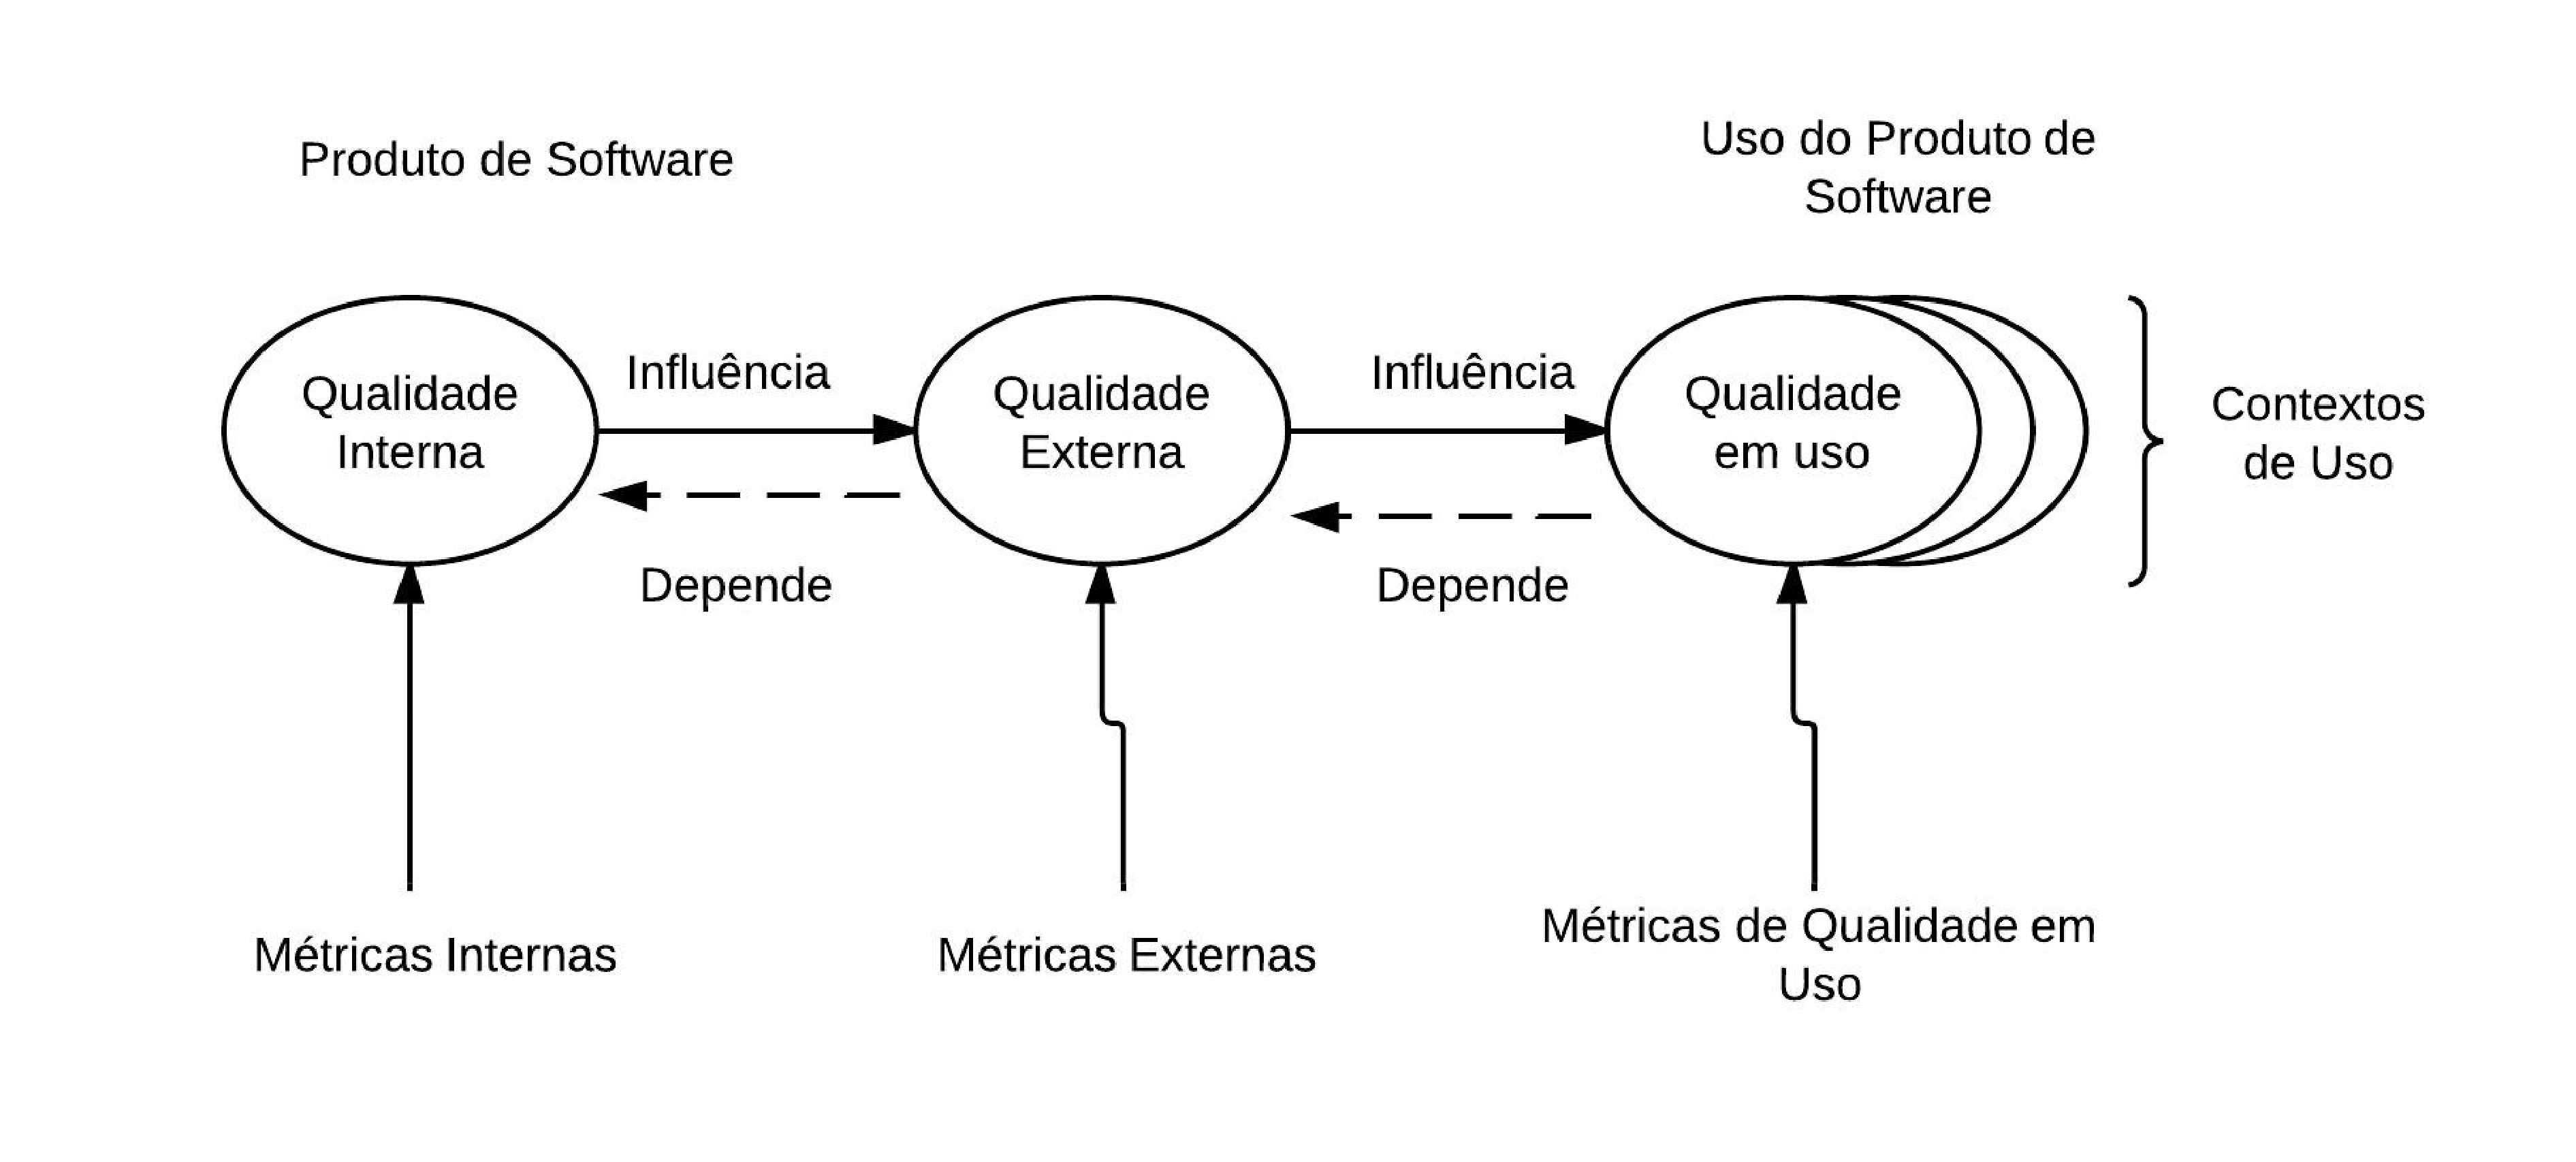
\includegraphics[keepaspectratio=false,scale=1.0]{figuras/modelodequalidade.eps}
		\caption{Modelo de Qualidade do Produto da ISO 25023}
		\label{modelodequalidade}
	\end{figure}
			
		\begin{description}
		\item[Métricas Internas.] 
		São métricas que aferem a qualidade interna do software que é avaliação de estruturas internas que compõem o software em estágio de desenvolvimento.  São exemplos de atributos da qualidade interna: simplicidade, concisão, coesão, clareza, baixo acoplamento e generalidade. 
			
		\item[Métricas Externas.]
		São métricas que capturam o comportamento do software. Exemplos de atributos da qualidade externa: correção, usabilidade, eficiência e robustez. qualidade externa mede  o comportamento do software. Estas só podem ser aferidas por atividades de teste do desenvolvimento do software em condições similares as que serão encontradas em ambientes de implantação.
			
		\item[Métricas de Qualidade em Uso.]
		 São métricas que aferem se o software atende as necessidades do cliente com eficiência, produtividade, segurança e satisfação em contextos específicos de uso. Estas só podem ser coletadas em ambientes reais, isto é, o ambiente o qual fora previamento projetado.
			 
		\end{description}
		
		 Conforme a figura \ref{modelodequalidade} mostra que ao investirmos em melhoria de qualidade interna do produto, provalmente trará benefícios tanto qualidade externa quanto na qualidade em uso. Este fato fica claro quando \citeonline{beckarticle1999} elucida que quando para reduzir o tempo de entrega, torcendo que a qualidade externa não sofra muito, é jogada tentadora para se evitar o caos de algumas semanas e meses no projeto reduzir a qualidade interna. Contudo, no final os problemas de qualidade interna aparecem e o software torna-se extremamente caro de ser mantido, ou incapaz de alcancar um nível competitivo de qualidade externa. 



%---------------------------------------------------------------------------------------------------------------------%
	
	\section {Métricas de Código-Fonte}
	\label {Métricas de Código-Fonte}
	
	\citeonline{Mills:1999} define que o produto de software deve ser entendido como um objeto abstrato que evolui de um conjunto inicial de necessidades até o sistema software acabado, incluindo o código-fonte e várias outras formas de documentação.
	
	Segundo a chamada de trabalhos do SCAM 2013~\footnote{13th IEEE International Working Conference on Source Code Analysis and Manipulation}, código-fonte é  qualquer descrição completamente executável de um sistema de software, desde de linguagem de máquina até representações gráficas executáveis.
	

	Segundo \citeonline{Sommerville10}, há duas formas de executar verificação e validação no código-fonte:
	
	\begin{description}
	
	\item[Estática.] A forma estática de avaliação do código-fonte é o meio pelo qual se pode analisar as estruturas internas do código sem realizar sua execução \cite{Wichmann95} e \cite{Nielson:1999}. Popularmente, o termo análise estática de código se refere uma análise automatizada, que é uma das técnicas estáticas de inspeção de software para obtenção de métricas de código-fonte \cite{Terra2008} \cite{Emanuelsson2008}.

	\item[Dinâmica.] A forma dinâmica de avaliação do código-fonte requer a execução da implementação. Os testes de software são técnicas que compreendem a abordagem de verificação dinâmica, podendo ser estes o teste de defeitos que tem a finalidade de encontrar inconsistências entre um programa e sua especificação, isto é, revelar defeitos e o teste de validação que tem a finalidade de mostrar que o software tem o comportamento que o cliente deseja \cite{Sommerville10}. 

	\end{description}

		Tendo como base a seção \ref{Classificação das Métricas}, métricas de código-fonte podem ser classificadas em \textit{métricas internas de produto}, quando obtidas por meio estáticos tal como a análise estática do código-fonte e \textit{métricas externas de produto}, quando obtidas por resultados de testes de software. As duas categorias podem ser classificadas em \textit{métricas objetivas}, pois o método de medição, tanto para métricas internas quanto externas, é definido por meio de regras matemáticas que são, em sua grande maioria, automatizadas em sua forma de coleta.

%-------------------------------------------------------------------------------------------------------------------------------------------------------------------%
	\subsection {Métricas Internas de Código-Fonte}
	\label {Métricas Internas de Código-Fonte}

	Esta subseção traz a classificação de métricas internas de código-fonte em subcategorias:

	\begin{description}
	\item [Tamanho.]  O tamanho do código-fonte foi uma das primeiras categorias a ser concebida, dado que o software poderia ocupar espaço tanto em forma de cartões perfurados quanto em forma de papel quando o código-fonte é impresso. A seção \ref{metrica tamanho} apresenta as principais métricas de tamanho. 

	\item [Complexidade.] A primeira lei de \citeonline{Lehman1980b} diz que um software deve ser continuamente adptado, se não a satisfação cai progressivamente.  Contudo a segunda lei de \citeonline{Lehman1980b} enuncia que a complexidade aumenta à medida que o software é evoluído, a menos que seja um trabalho de manutenção. Logo é perceptível que as métricas de complexidadde estão diretamente ligadas as métricas de tamanho, sendo a modificação em uma provavelmente impactará na outra. A seção \ref{metrica complexidade} apresenta as principais métricas de complexidade.

	\item [Paradigma de Programação.] A evolução dos paradigmas de programação permitiu que as linguagens de programação, assumissem diversas características entre si. O paradgima funcional, por exemplo, enxerga o programa como uma sequência de funções que podem ser executadas em modo funcional. Já o paradigma orientado a objetos visa abstrair as unidades computacionais em Classes, que representam em grande parte do desenvolvimento unidades reais, e partir destas abstrair instâncias computacionais, isto são, objetos propriamente ditos. Para cada paradigma, são necessárias métricas específicas. A seção \ref{metrica objetos} apresenta as principais métricas do paradigma orientado a objetos, pois este ainda é o paradigma mais utilizado no mercado de desenvolvimento de software. 
	\end{description}

\subsubsection{Métricas de Tamanho}
\label{metrica tamanho} 
	
	\begin{description}
	\item[LOC - Linhas de Código.] O LOC (do inglês Lines of Code) foi uma das primeiras métricas para medir o tamanho do software. É utilizada para contabilizar linhas que possuem instruções e não são brancas ou comentadas. 
	\end{description}

LOC é uma métrica simples de entender e fácil de computar, mas possui sérias limitações, pois pois cada linguagem de programação valoriza
de forma diferente clareza e brevidade, podendo diferir muito em verbosidade. Comparar linhas de
código de linguagens diferentes exige certos cuidados: podem ser usados fatores de normalização, ou
a comparação pode ser feita apenas em escala logarítmica. Projetos de software frequentemente são
desenvolvidos usando mais de uma linguagem de programação. Como não é razoável simplesmente
somar, fica difícil definir medidas como erros por linhas de código. (Carlos Morais)



\subsubsection {Métricas de Complexidade}
\label {metrica complexidade}


\subsubsection{Métricas Orientadas à Objetos}
\label{metrica objetos}






